\documentclass[10pt,letterpaper]{article}
\usepackage{graphicx} % Required for inserting images
%\topmargin -.45in
\textwidth 6.5in
\textheight 9.in
\oddsidemargin 0in
\headheight 0in
\usepackage{subfig}
\usepackage{float}
\usepackage{fancybox}
% \usepackage{p alatino}
\usepackage[utf8]{inputenc} %solucion del problema de los acentos.
\usepackage{epsfig}
\usepackage{multicol,pst-plot}
\setlength{\columnsep}{5mm}
\usepackage{pstricks}
\usepackage{amsmath}
\usepackage{amsfonts}
\usepackage{amssymb}
\usepackage{eucal}
\usepackage[left=2cm,right=2cm,top=2cm,bottom=2cm]{geometry}
\pagestyle{empty}
\DeclareMathOperator{\tr}{Tr}
\newcommand*{\op}[1]{\check{\mathbf#1}}
% \newcommand{\bra}[1]{\langle #1 |}
% \newcommand{\ket}[1]{| #1 \rangle}
\newcommand{\braket}[2]{\langle #1 | #2 \rangle}
\newcommand{\mean}[1]{\langle #1 \rangle}
\newcommand{\opvec}[1]{\check{\vec #1}}
\renewcommand{\sp}[1]{$${\begin{split}#1\end{split}}$$}
\usepackage{hyperref}       % hyperlinks
\usepackage{url}            % simple URL typesetting
\usepackage{booktabs}       % professional-quality tables
\usepackage{amsfonts}       % blackboard math symbols
\usepackage{nicefrac}       % compact symbols for 1/2, etc.
\usepackage{microtype}      % microtypography
\usepackage{lipsum}
\usepackage[spanish, es-tabla]{babel}
\usepackage{amssymb}
\usepackage{fancyhdr}
\usepackage[nottoc]{tocbibind}
\usepackage[titletoc]{appendix}
\usepackage{fancyhdr}
\usepackage{multirow}
\usepackage{subfigure}
\usepackage{csquotes}
\usepackage{csquotes}
\usepackage{multicol}
\usepackage{cancel}
\usepackage{mathtools}
\usepackage{amssymb}
\usepackage{parskip}
\usepackage{amsthm}
\usepackage{amsmath}
\usepackage{titlesec}
\usepackage{float}
\graphicspath{{images/}}
\renewcommand{\labelitemii}{$\ast$}
\providecommand{\abs}[1]{\lvert#1\rvert}
\providecommand{\norm}[1]{\lVert#1\rVert}
\usepackage{subcaption}
\usepackage{listings}
\usepackage{color}

\definecolor{codegreen}{rgb}{0,0.6,0}
\definecolor{codegray}{rgb}{0.5,0.5,0.5}
\definecolor{codepurple}{rgb}{0.58,0,0.82}
\definecolor{backcolour}{rgb}{0.95,0.95,0.92}

\lstdefinestyle{mystyle}{
	backgroundcolor=\color{backcolour},   
	commentstyle=\color{codegreen},
	keywordstyle=\color{magenta},
	numberstyle=\tiny\color{codegray},
	stringstyle=\color{codepurple},
	basicstyle=\footnotesize,
	breakatwhitespace=false,         
	breaklines=true,                 
	captionpos=b,                    
	keepspaces=true,                 
	numbers=left,                    
	numbersep=5pt,                  
	showspaces=false,                
	showstringspaces=false,
	showtabs=false,                  
	tabsize=2
}

\usepackage{authblk}
\author[1]{Castiblanco D.}
\author[2]{Velazquez G.}
\author[3]{Ruiz J.}
\author[4]{Rodriguez M.}
\affil[1, 2, 3, 4]{Departmento de física\\
Universidad Nacional de Colombia - Bogotá}


\title{ \Huge Rectificadores}
\date{17 de noviembre de 2023}

\begin{document}

\maketitle

\begin{center}\rule{\textwidth}{0.1mm}\end{center}
\begin{center}\vspace{0.2cm}

	\begin{abstract}
		A partir de un transformador, se observa el funcionamiento de tres rectificadores distintos (con 1, 2, 4 diodos) a los cuales se les añadio una resistencia y en el ultimo caso, una capasitancia para obtener un rizado de filrtrado.

	\end{abstract}

\end{center}


\begin{center}\rule{\textwidth}{0.1mm}\end{center}

\section{Análisis}

\subsection{Onda Media}

Se inicia caracterizando el primer rectificador, al cual se le pone un solo diodo de alta frecuencia (Diodo de alta frecuencia) que actúa como una fuente de onda media.
Se usa tambien, un transformador configurado con 120 V de entrada de corriente alterna,
y una resistencia de $5$ KiloOhms para generar la onda media en el circuito.
\\ El diagrama de la red es como se muestra a continuación:

\begin{figure}[H]
	\centering
	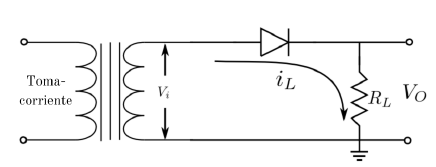
\includegraphics[scale=1.5]{OndaMedia.png}
	\caption{Circuito para la caracterización de rectificador onda media con un diodo.}
	\label{salida}
\end{figure}

La señal obtenida en el osciloscopio se muestra a continuación

\begin{figure}[H]
    \centering
    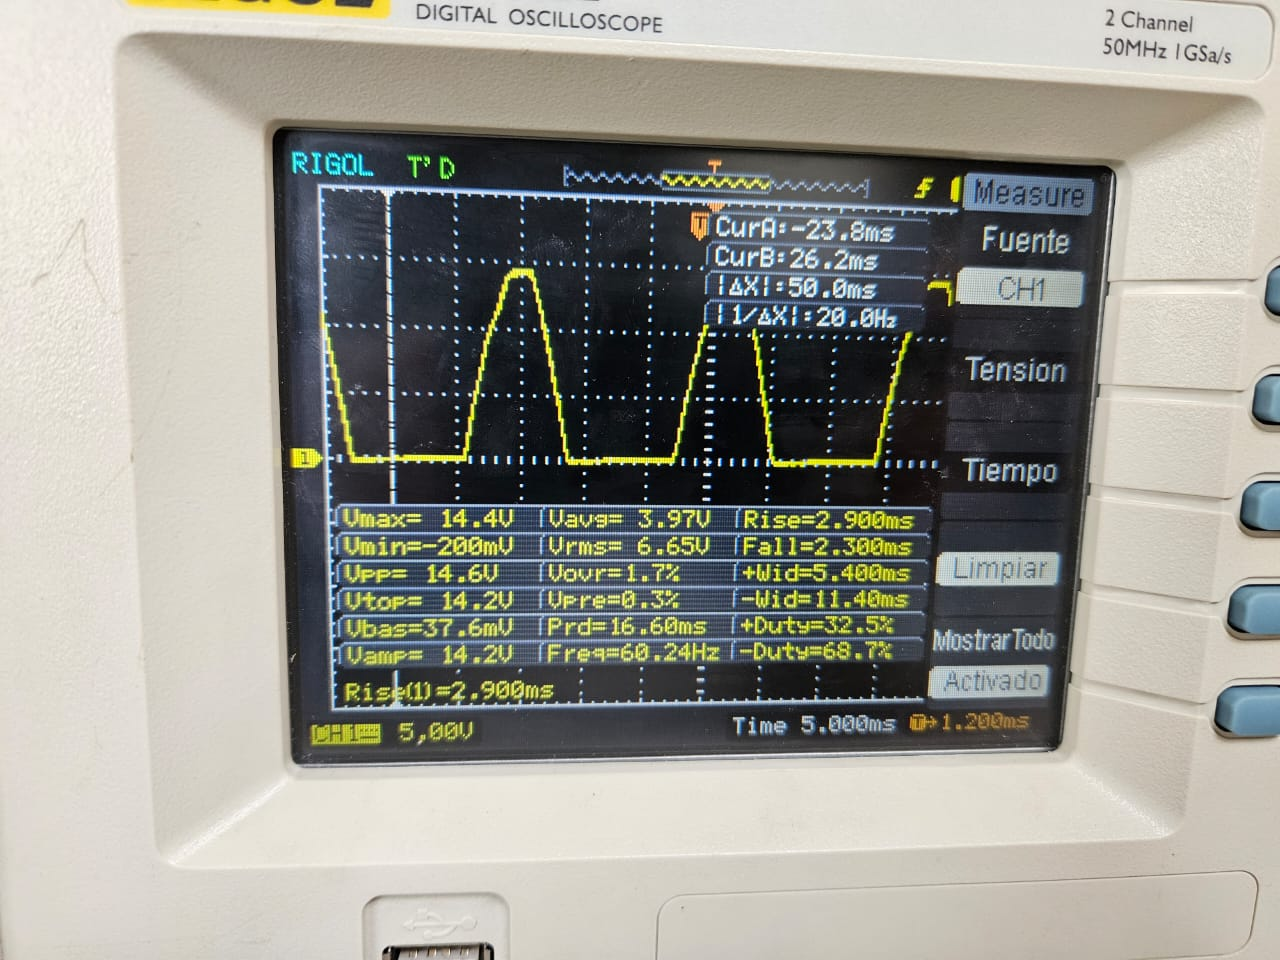
\includegraphics[scale=0.387]{Osc_OndaMedia.jpg}
    \caption{Señal de rectificador de onda media}
    \label{SeñalMedia}
\end{figure}

Por lo que se observa en los gráficos anteriores, la señal tiene dos componentes principales,
la parte positiva y negativa del sinal de corriente alterna. La señal positiva es la suma de las
dos mitades de la señal completa, mientras que la señal negativa es la diferencia entre ambas
mitades. Esto ocurre porque el diodo no permite pasar la corriente hacia abajo, por lo tanto, solo
permite que fluya desde arriba hacia abajo, pero no viceversa. Por esta razón, al aplicar la
corriente alterna a través del diodo, solo se obtiene la mitad de la señal completa.\\

En la imagen, se evidencia que la medida de la señal $V_p=14.4 V$, donde el valor de la escala
por division es de $5V$.\\

El proceso se repite en las siguientes secciones para  cada uno de los rectificadores.



\subsection{Onda Completa}

Para realizar la caracterización de rectificador de onda completa, se utiliza un transformador
configurado con 120 V de entrada de corriente alterna, y una resistencia de $5$ KiloOh
ms para generar la onda completa en el circuito. \\ El diagrama de la red es como se muestra
a continuación:

\begin{figure}[H]
	\centering
	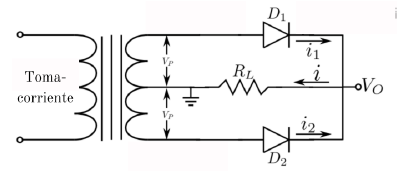
\includegraphics[scale=1.2]{OndaCompleta2.png}
	\caption{Circuito para la caracterización de rectificador onda completa con dos diodos.}
	\label{fig:OndaCompleta2}
\end{figure}

La señal obtenida en el osciloscopio se muestra a continuación

\begin{figure}[H]
	\centering
	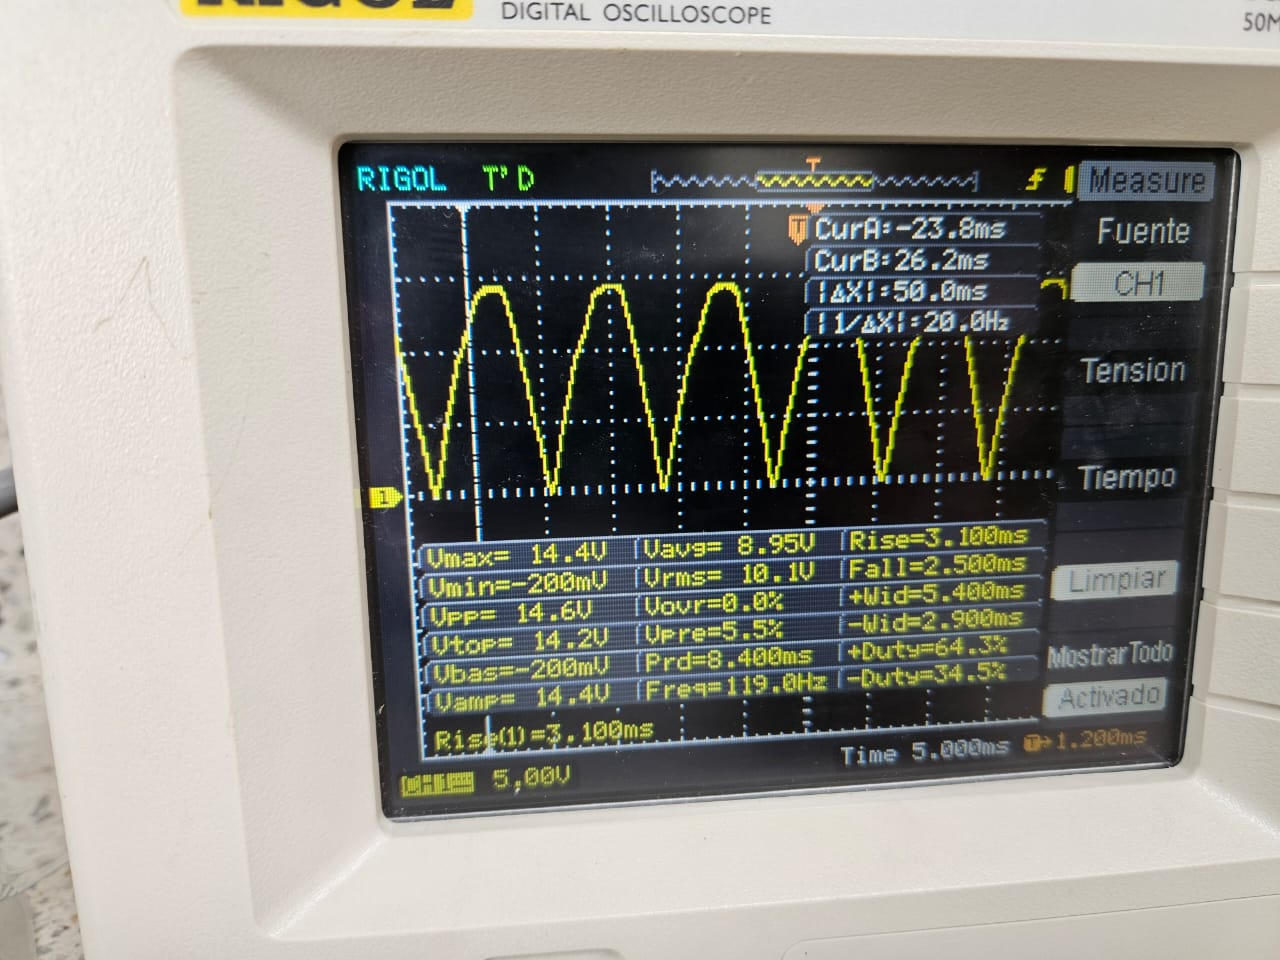
\includegraphics[scale=.35]{Osc_OndaCompleta.jpg}
	\caption{Señal de rectificador de onda completa con dos diodos}
	\label{fig:OndaCompleta}
\end{figure}

Como se puede ver en los gráficos anteriores, la señal tiene tres componentes principales,
la parte positiva y negativa del sinal de corriente alterna, y la tercera componente es la
parte intermedia de la señal. En este caso, la señal completa es la suma de las dos partes
positivas y negativas. Es decir, la señal completa es la suma de la señal positiva y la
negación de la señal negativa.\\
Es importante destacar que el rectificador de onda completa es capaz de producir una señal
completa sin necesidad de utilizar un capacitor.\\
En la imagen, se evidencia que la medida de la señal $V_p=14.4 V$ (similar al valor de onda media), donde
el valor de la escala por division es de $5V$ y se ve que varia el periodo de la señal respecto a la mostrada por el rectificador de onda media.\\

Por otra parte, para el rectificador de onda completa de cuatro diodos se tiene el siguiente circuito:
\begin{figure}[H]
	\centering
	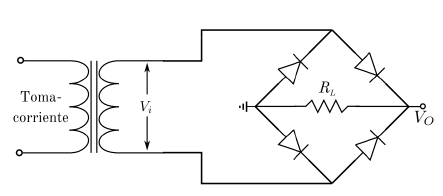
\includegraphics[scale=1]{OndaCompleta4.png}
	\caption{Circuito para la caracterización de rectificador onda completa con cuatro diodos}
	\label{fig:4}
\end{figure}
Y su señal respectiva tiene la forma:

\begin{figure}[H]
	\centering
	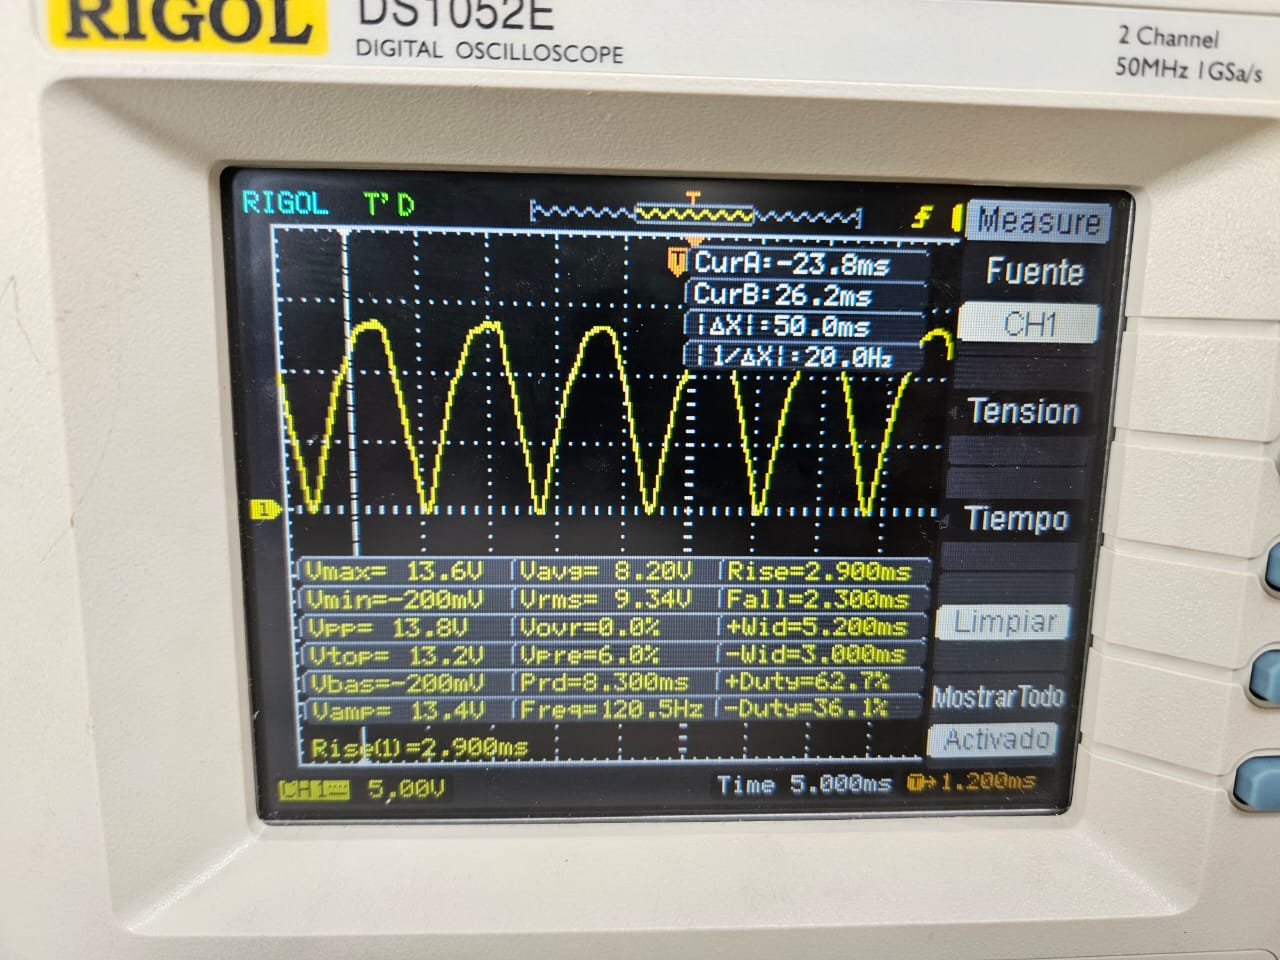
\includegraphics[scale=.35]{Osc_OndaCompleta4D.jpg}
	\caption{Señal de rectificador de onda completa con cuatro diodos}
	\label{fig:4D}
\end{figure}

El resultado de esta configuración es similar al anterior, pero con la ventaja de tener una mayor
capacidad de absorber energía por medio de los diodos. Por ello el valor de $V_p=13.6 V$, un poco menor que para dos diodos\\


\subsection{Rizado de Filtrado}

El ultimo circuito, siendo el mas complejo, posee un capacitor el cual 
se utiliza como filtro pasabajas para reducir la frecuencia de salida. El capacitor
funciona como un condensador eléctrico, lo que permite controlar la impedancia de salida
del circuito. La función principal del capacitor es eliminar la frecuencia de corte,
lo que reduce la distorsión en la señal de salida.

\begin{figure}[H]
	\centering
	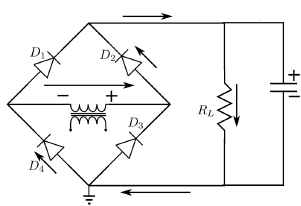
\includegraphics[scale=1]{OndaCapacitorFiltrado.png}
	\caption{Circuito para la caracterización de rectificador onda completa con cuatro diodos y capacitor de filtrado}
	\label{fig:filtrado}
\end{figure}

La señal resultante es la suma de la señal completa y la señal de rizado de filtrado.

Para este circuito, se opto por medir primeramente la resistencia fija de 10 $k\Omega$ en el cual se obtienen las imagenes mostradas en la figura \ref{fig:cuadricula}, de las cuales bastantes tuvieron que despreciarse para evitar el ruido en los datos para los cuales se obtuvieron las graficas siguientes. Se evidencia que a medida que aumenta el voltaje promedio y de rizado el porcentaje de rizado se hace mayor.

\begin{figure}[H]
    \centering
    \begin{minipage}[b]{0.45\textwidth}
        \centering
        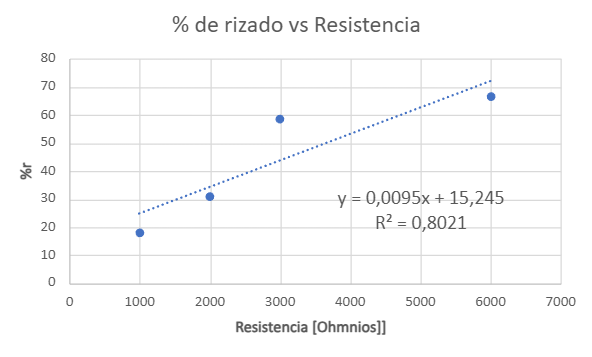
\includegraphics[scale=0.65]{FiltradoResitencia_plt.png}
        \caption*{\% Filtrado vs Resistencia}
    \end{minipage}
            \begin{minipage}[b]{0.45\textwidth}
        \centering
        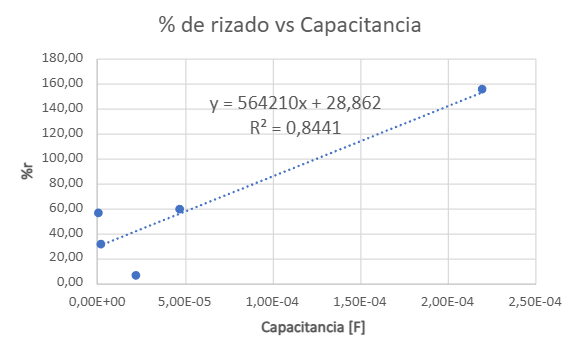
\includegraphics[scale=0.65]{FiltradoCapacitancia_plt.png}
        \caption*{\% Filtrado vs Capacitancia}
    \end{minipage}
    \caption{Caption}
    \label{fig:enter-label}
\end{figure}



\begin{figure}[H]
    \centering
    \begin{minipage}[b]{0.45\textwidth}
        \centering
        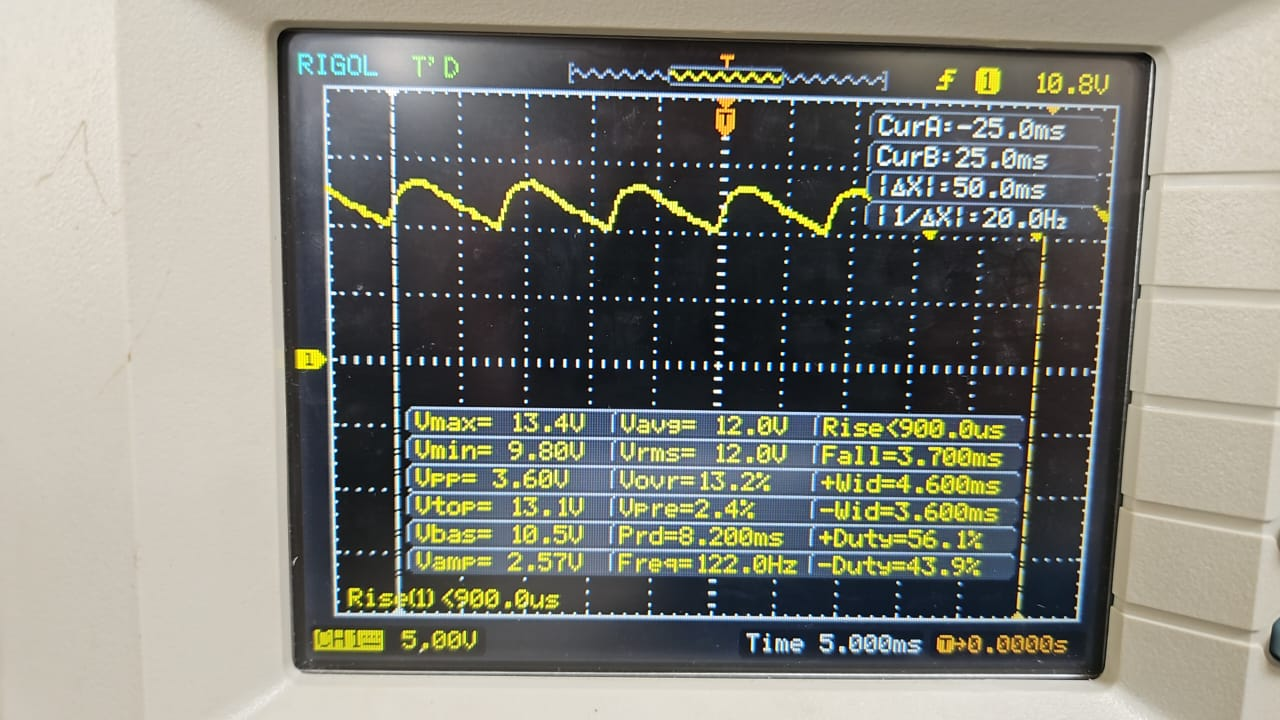
\includegraphics[scale=0.2]{Filtrado0.jpg}
        \caption*{a}
    \end{minipage}
    \hfill
    \begin{minipage}[b]{0.45\textwidth}
        \centering
        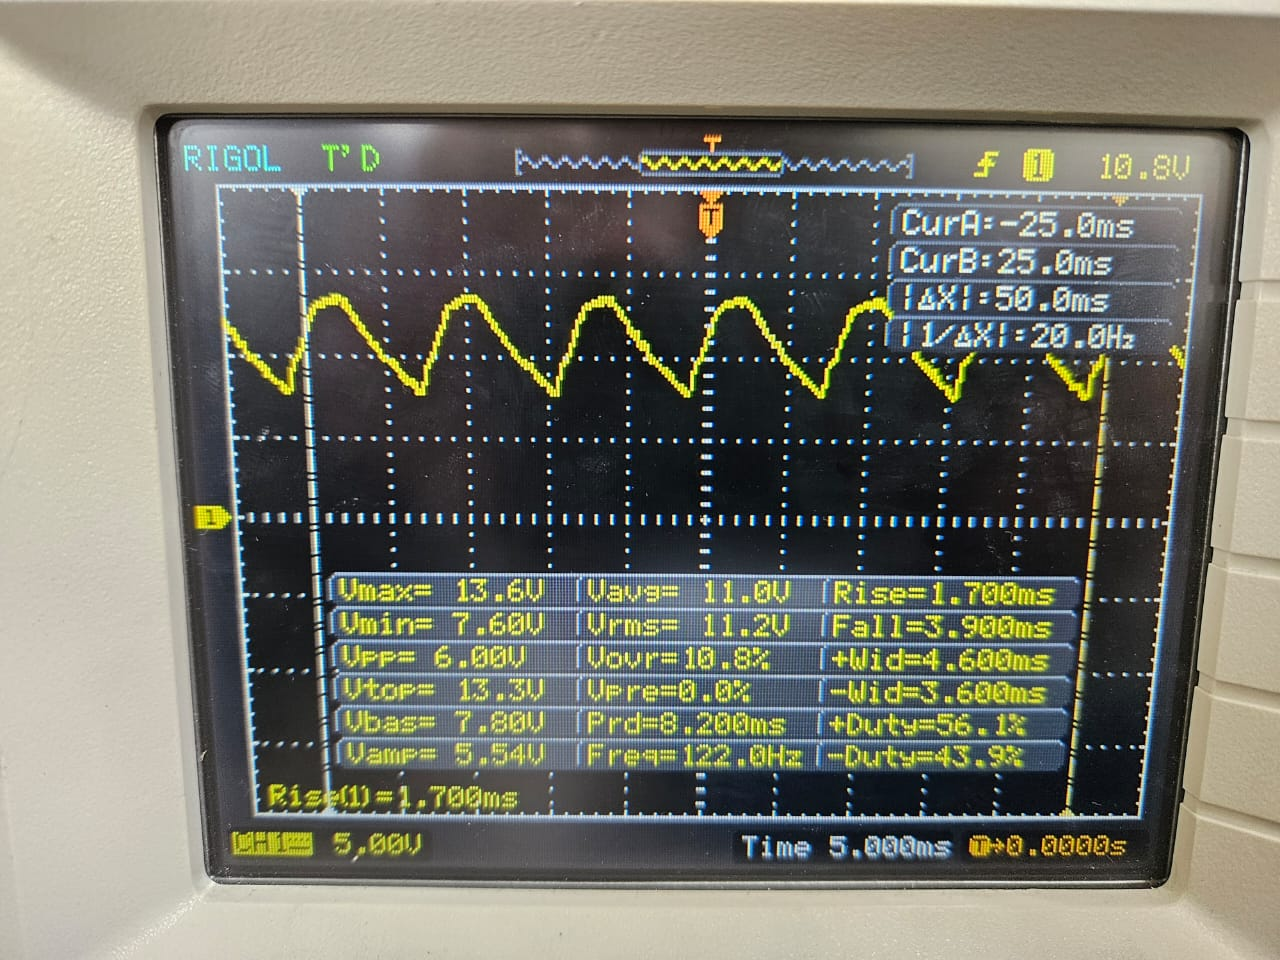
\includegraphics[scale=0.15]{Filtrado7.jpg}
        \caption*{b}
    \end{minipage}
    \\

    \hfill
    \begin{minipage}[b]{0.45\textwidth}
        \centering
        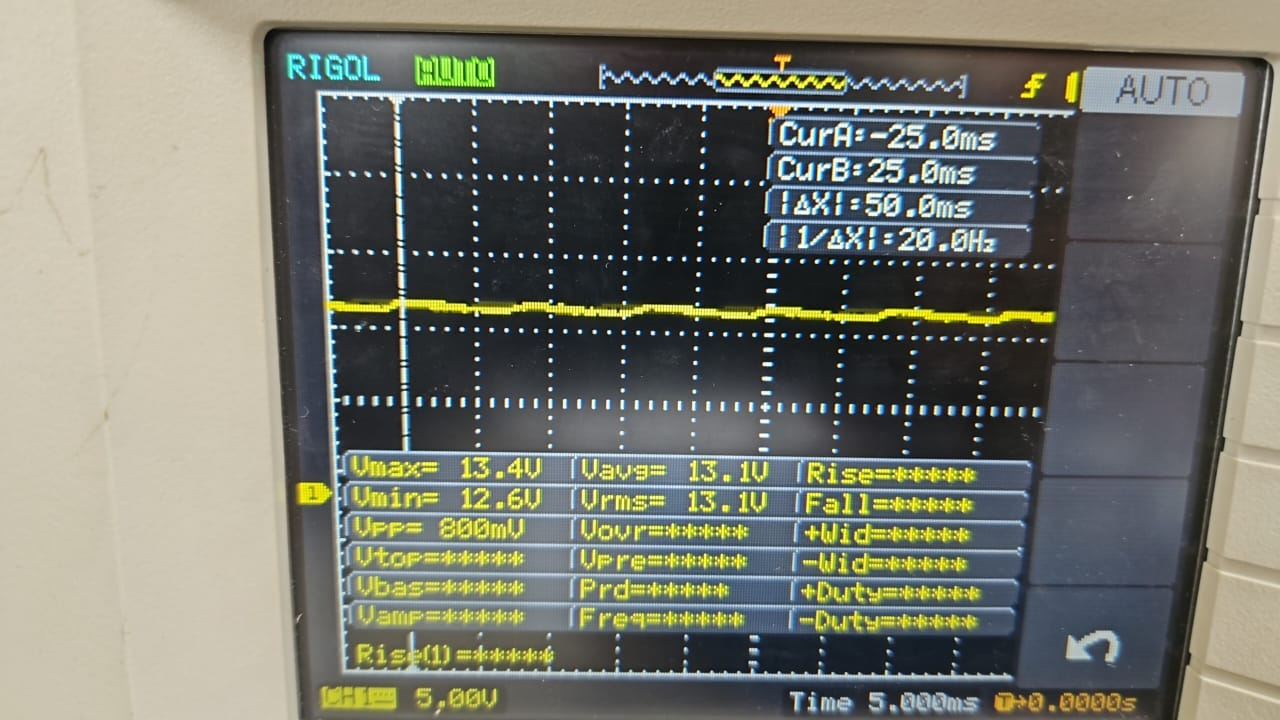
\includegraphics[scale=0.2]{Filtrado9.jpg}
        \caption*{d}
    \end{minipage}
    \hfill
        \begin{minipage}[b]{0.45\textwidth}
        \centering
        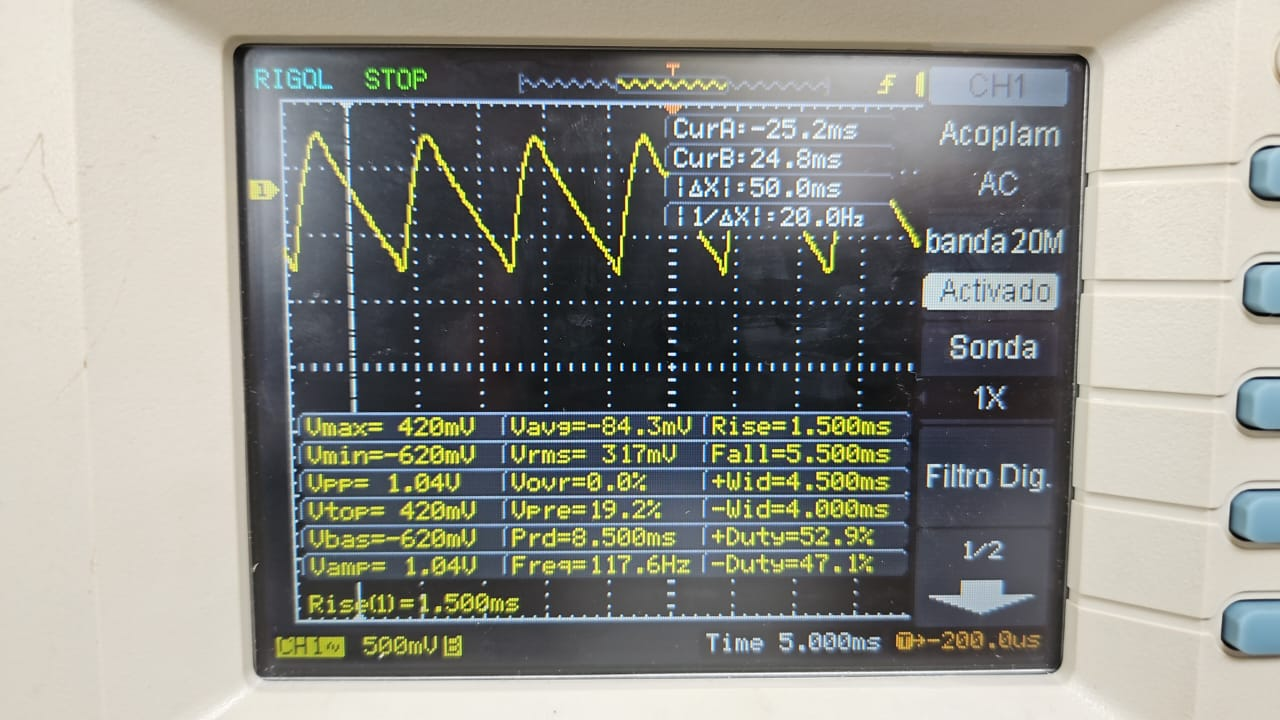
\includegraphics[scale=0.2]{Filtrado4.jpg}
        \caption*{e}
    \end{minipage}
    \hfill
        \begin{minipage}[b]{0.45\textwidth}
        \centering
        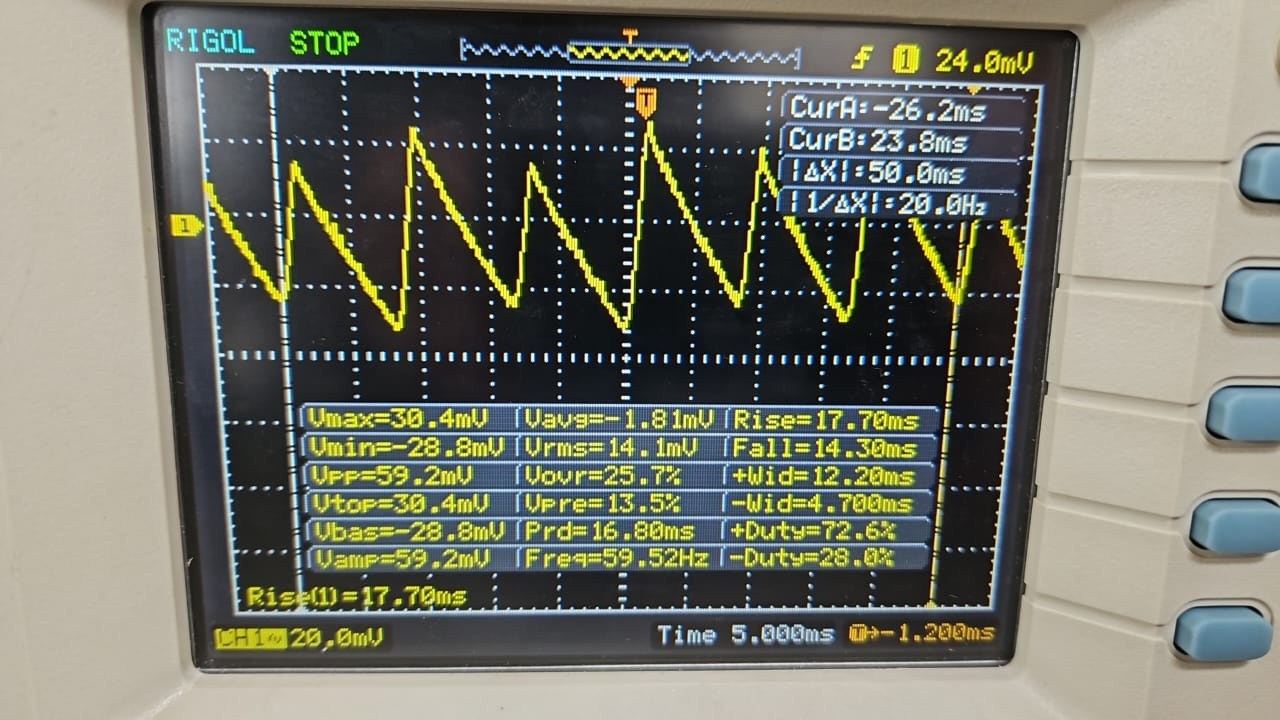
\includegraphics[scale=0.2]{Filtrado5.jpg}
        \caption*{f}
    \end{minipage}
    \caption{Rizado de filtrado variando la capacitancia.}
    \label{fig:cuadricula}
\end{figure}

\begin{figure}[H]
    \centering
        \begin{minipage}[b]{0.45\textwidth}
        \centering
        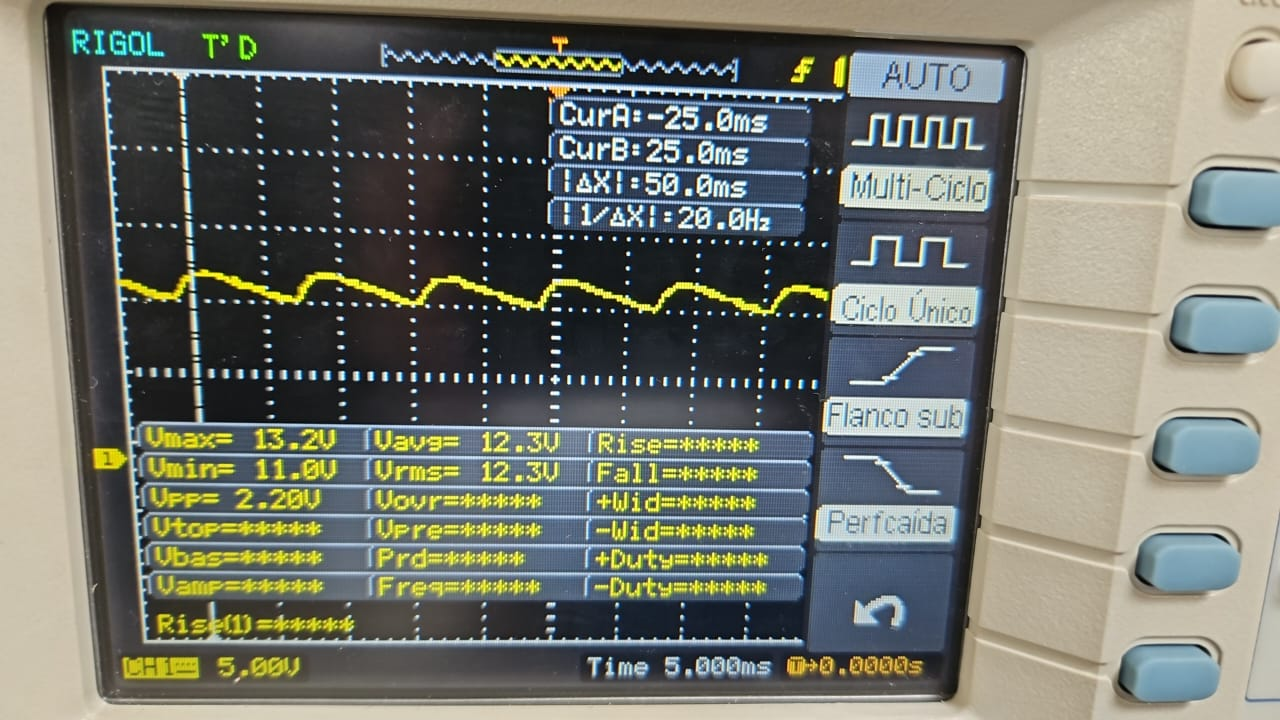
\includegraphics[scale=0.2]{Filtrado8.jpg}
        \caption*{a}
    \end{minipage}
    \begin{minipage}[b]{0.45\textwidth}
        \centering
        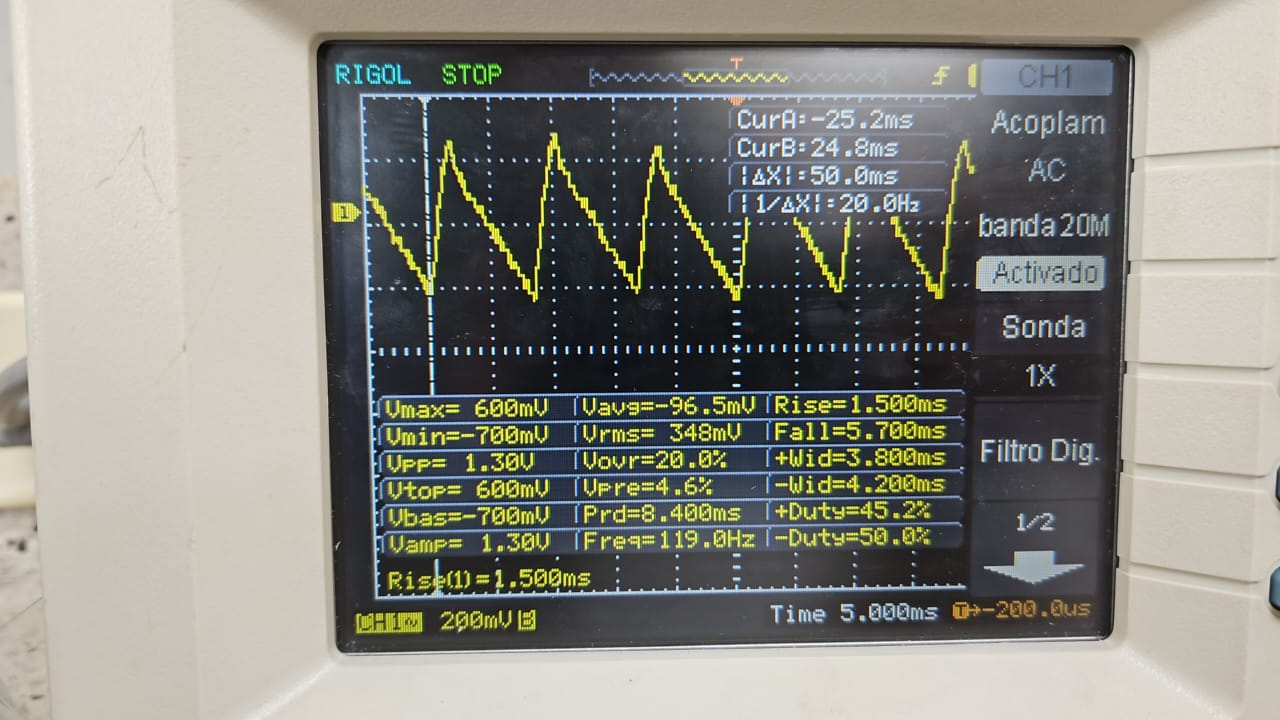
\includegraphics[scale=0.2]{Filtrado1.jpg}
        \caption*{b}
    \end{minipage}    
    \hfill
    \begin{minipage}[b]{0.45\textwidth}
        \centering
        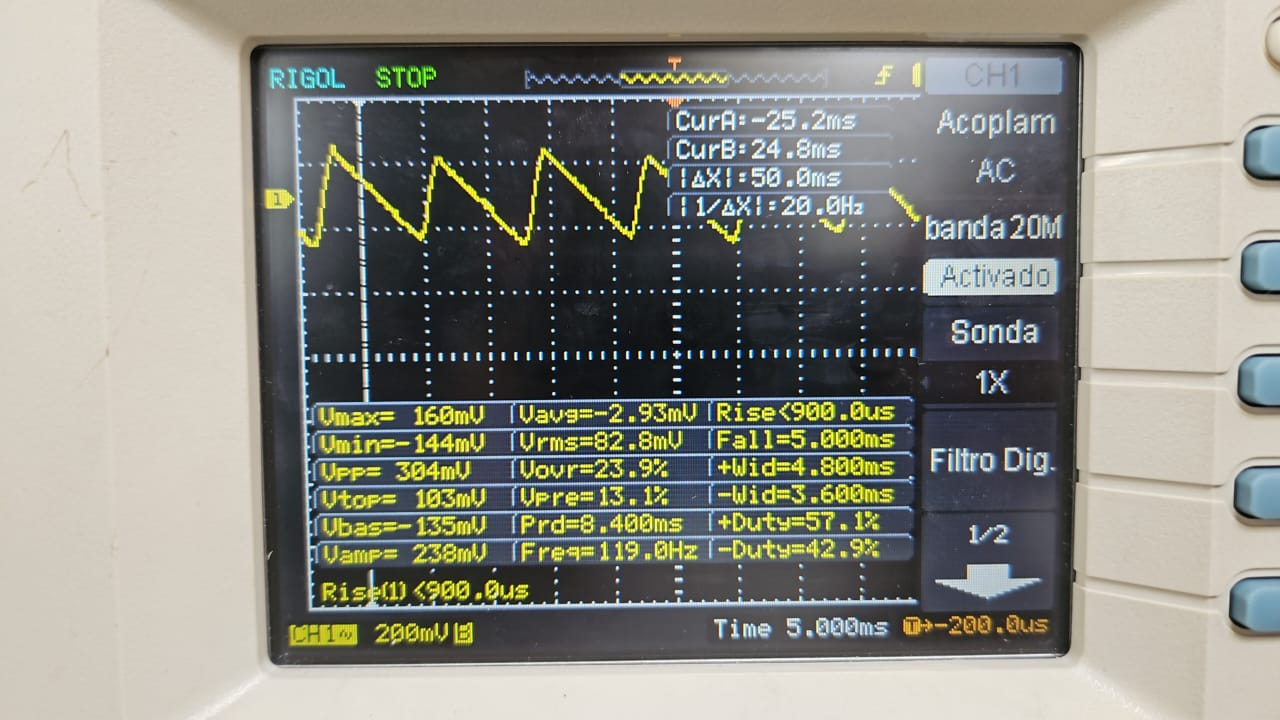
\includegraphics[scale=0.2]{Filtrado2.jpg}
        \caption*{c}
    \end{minipage}
    \begin{minipage}[b]{0.45\textwidth}
        \centering
        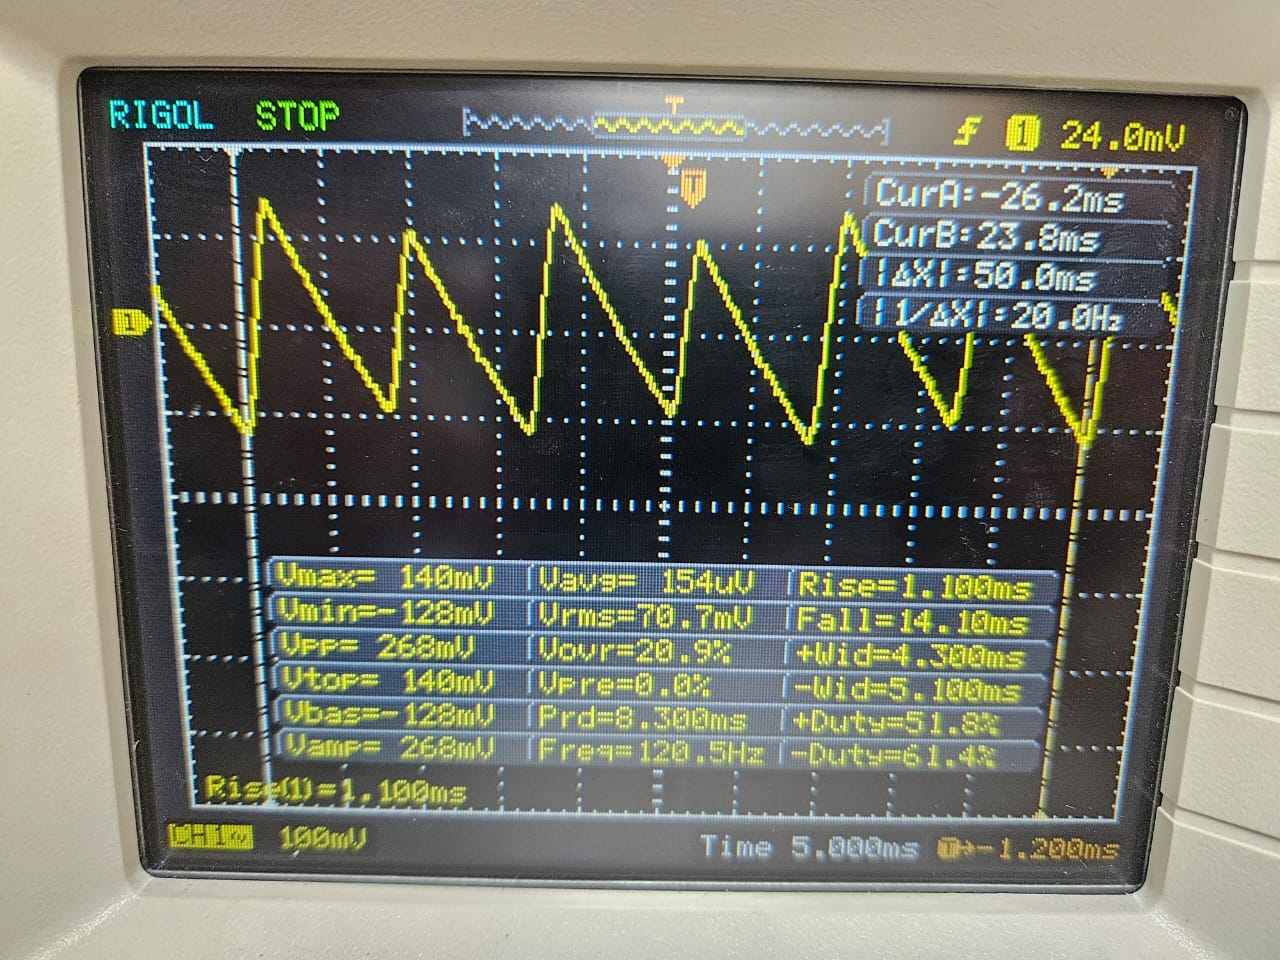
\includegraphics[scale=0.15]{Filtrado6.jpg}
        \caption*{d}
    \end{minipage}
    \caption{Caption}
    \label{fig:enter-label}
\end{figure}


\section{Conclusiones}
\begin{itemize}
	\item








\end{itemize}

\begin{thebibliography}{9}
	% àdfasdfasd
\end{thebibliography}

\end{document}
